%%%%%%%%%%%%%%%%%%%%%%%%%%%%%%%%%%%%%%%%%%%%%%%%%%%%%%%%%%%%%%%%%%%%%
%
%  This is a sample LaTeX input file for your contribution to 
%  the MC2013 conference. Modified by R.C. Martineau at INL from A. 
%  Sood at LANL, from J. Wagner ORNL who obtained the original class 
%  file by Jim Warsa, LANL, 16 July 2002}
%
%  Please use it as a template for your full paper 
%    Accompanying/related file(s) include: 
%       1. Document class/format file: mc2013.cls
%       2. Sample Postscript Figure:   figure.eps
%       3. A PDF file showing the desired appearance: template.pdf 
%    Direct questions about these files to: richard.martinea@inl.gov
%
%    Notes: 
%      (1) You can use the "dvips" utility to convert .dvi 
%          files to PostScript.  Then, use either Acrobat 
%          Distiller or "ps2pdf" to convert to PDF format. 
%      (2) Different versions of LaTeX have been observed to 
%          shift the page down, causing improper margins.
%          If this occurs, adjust the "topmargin" value in the
%          mc2013.cls file to achieve the proper margins. 
%
%%%%%%%%%%%%%%%%%%%%%%%%%%%%%%%%%%%%%%%%%%%%%%%%%%%%%%%%%%%%%%%%%%%%%


%%%%%%%%%%%%%%%%%%%%%%%%%%%%%%%%%%%%%%%%%%%%%%%%%%%%%%%%%%%%%%%%%%%%%
\documentclass{mc2013}
%
%  various packages that you may wish to activate for usage 
\usepackage{graphicx}
\usepackage{tabls}
\usepackage{afterpage}
\usepackage{cites}
\usepackage{color}
\usepackage{amsmath,amsthm,amssymb}
\usepackage{verbatim}
\usepackage[parfill]{parskip}
\usepackage{tikz}
\usepackage{subcaption}
\usepackage[labelfont=bf]{caption}
 
\newcommand{\N}{\mathbb{N}}
\newcommand{\Z}{\mathbb{Z}}
\newcommand{\deriv}[2]{\frac{\mathrm{d} #1}{\mathrm{d} #2}}
\newcommand{\pderiv}[2]{\frac{\partial #1}{\partial #2}}
\newcommand{\bx}{\mathbf{X}}
\newcommand{\ba}{\mathbf{A}}
\newcommand{\by}{\mathbf{Y}}
\newcommand{\bj}{\mathbf{J}}
\newcommand{\bs}{\mathbf{s}}
\newcommand{\B}[1]{\ensuremath{\mathbf{#1}}}
\newcommand{\Dt}{\Delta t}
\renewcommand{\d}{\mathrm{d}}
\newcommand{\mom}[1]{\langle #1 \rangle}
\newcommand{\xl}{{x_{i-1/2}}}
\newcommand{\xr}{{x_{i+1/2}}}
\newcommand{\il}{{i-1/2}}
\newcommand{\ir}{{i+1/2}}

\graphicspath{{figures/}}
 
%\usepackage{epsf}
%
%
% Insert authors' names and short version of title in lines below
%
\newcommand{\authorHead}      % Author's names here
   {S.R. Bolding and J.E. Morel}  
\newcommand{\shortTitle}      % Short title here
   {A HOLO method with ECMC for Thermal Radiative Transfer}  
%%%%%%%%%%%%%%%%%%%%%%%%%%%%%%%%%%%%%%%%%%%%%%%%%%%%%%%%%%%%%%%%%%%%%
%
%   BEGIN DOCUMENT
%
%%%%%%%%%%%%%%%%%%%%%%%%%%%%%%%%%%%%%%%%%%%%%%%%%%%%%%%%%%%%%%%%%%%%%
\begin{document}

%
%      Headers and Footers
\afterpage{%
\fancyhf{}%
\fancyhead[CE]{              
{\scriptsize \authorHead}}                                                
\fancyhead[CO]{               
{\scriptsize \shortTitle}}                  
%\lfoot{\scriptsize{
%International Conference on Mathematics and Computational Methods
%Applied to Nuclear Science \& Engineering (M\&C 2013), 
%\\ Sun Valley, Idaho, USA, May 5-9, 2013.}}%
\rfoot{\thepage/\totalpages{}}%

\pagestyle{fancy}
%\setlength{\topmargin}{-20pt}
}
 
\normalsize

\setlength{\baselineskip}{16.8pt}
\vspace{-3pt}

% 
% TITLE
%

\begin{center}
\textbf{\large \\%
A HIGH-ORDER LOW-ORDER ALGORITHM WITH EXPONENTIALLY-CONVERGENT MONTE CARLO FOR
THERMAL RADIATIVE TRANSFER\\
}
% 
% FIRST AUTHORS 
%
\setlength{\baselineskip}{14pt}
\textbf{S.R. Bolding and J.E. Morel} \\
Department of Nuclear Engineering\\
Texas A\&M University  \\
College Station, TX 77843 \\
sbolding@tamu.edu; morel@tamu.edu \\

% 
% SECOND AUTHORS (if not needed delete from here) 
%
\vspace{12pt}
\textbf{CCS-2 people???}\\
Department of Nuclear Engineering  \\
Name of University \\
Address \\
C@name.univ.edu\\ 
%
% SECOND AUTHORS (to here)
%

\end{center}

%
% SET RAGGED RIGHT MARGIN
%
\raggedright


\section*{ABSTRACT} 
\begin{quote}
\begin{small}
We have implemented a new high-order low-order (HOLO) algorithm for solving
thermal radiative transfer (TRT) problems.  The low-order (LO) system is based on spatial
and angular moments of the transport equation and a linear discontinuous
finite-element spatial representation, producing equations similar to the standard
S$_2$ equations.  
The LO solver is fully implicit in time and efficiently resolves the non-linear
temperature dependence at each time step.   The HO solver
utilizes exponentially-convergent Monte Carlo (ECMC) to give a globally accurate solution
for the angular intensity to a fixed-source, pure absorber transport problem.  This global solution is used to compute consistency terms
that require the HO and LO solutions to converge to the same solution.  The use of ECMC
allows for efficient reduction of statistical noise in the MC solution, eliminating
inaccuracies introduced through the LO consistency
terms.  We compare results with an
implicit Monte Carlo (IMC) code for one-dimensional gray test problems and 
demonstrate the efficiency of ECMC over SMC in this algorithm.

\emph{Key Words}: List of at most five key words

\end{small} 
\end{quote}

\setlength{\baselineskip}{14pt}
\normalsize

\Section{INTRODUCTION}

We have implemented a high-order low-order (HOLO) algorithm for the case of gray, one spatial dimension
TRT problems. The governing equations are the radiation and
material energy balance equations, i.e.,
\begin{align}\label{ho_cont}
    \frac{1}{c}\pderiv{I}{t} + \mu \pderiv{I}{x} + \sigma_t I
&= \frac{\sigma_s}{2} \phi +\frac{1}{2} \sigma_a a c T^4
  \\
  \rho c_v \pderiv{T}{t} &= \int_{-1}^{1} \sigma_a I(x,\mu)
\d\mu - \sigma_a a c (T^4),
\end{align}
In the above equations $x$ is the position, $t$ is the time, $\mu$ is
the $x$-direction cosine of the angular intensity $I(x,\mu,t)$, and $a$, $c$, $\rho$,
and
$c_v$ are the radiation constant, speed of light, mass density, and specific heat; $\sigma_a$, $\sigma_s$, and
$\sigma_t$ are the absorption, scattering, and total
opacities (cm$^{-1}$), respectively. The desired fundamental unknowns are the material
temperature $T(x,t)$ and the scalar radiation intensity $\phi(x,t)=\int_{-1}^1
I(x,\mu,t) \d \mu$. The equations are
strongly coupled through the gray Planckian emission source $\sigma_a a c T^4$, which
is a nonlinear function of temperature, and the absorption
term $\sigma_a \phi$.   In general, the material properties are a function of $T$,
introducing additional non-linearity.  The non-linear material properties and
absorption-reemission physics lead to systems that require solution in a mix of
streaming and optically-thick, diffusive regions. 

Monte Carlo (MC) solution to the TRT equations is typically achieved by the 
implicit Monte Carlo (IMC) method, first introduced by Fleck and Cummings~\cite{fnc}. This
method linearizes the emission source in time to eliminate the material energy equation from the system. The remaining
transport equation contains an approximate emission source, as well as an effective scattering cross section representing
absorption and reemission over a time step.    In optically thick regions, or for
large time steps, the
effective scattering dominates interactions.  In these diffusive regions IMC
becomes computationally expensive. Additionally, the approximate linearization of the emission source is
not iterated on within a time step, limiting the time step size to produce physically
accurate results. 

Moment-based hybrid Monte Carlo (MC) methods provide an alternative solution
method.  Recent work has focused on fixed-point iteration high-order low-order (HOLO)
approaches~\cite{willert,park,rmc,ans_2014}.  Such methods utilize a low-order (LO)
operator based on angular moments of the transport equation, formulated over a coarse
spatial mesh. Physics operators that are time consuming for MC
to resolve, e.g., absorption-reemission and scattering events, are moved to the LO
system.  Newton methods allow for non-linearities in the LO equations to be fully
resolved efficiently~\cite{willert}.  The high-order (HO) system is defined by
Eq.~\eqref{ho_cont}, with sources estimated from the LO solution. The HO system is solved via MC to produce a high-fidelity solution for
the angular intensity.  The MC estimate of the angular intensity is used to estimate consistency terms,
present in the LO equations, that require the LO system to preserve the angular accuracy of the
MC solution; the HO system does not directly estimate a new material temperature,
eliminating stability issues that require linearization of the emission source.
However, sufficient MC histories must be performed to eliminate statistical
noise in the conistency terms, which can contaminate the LO solution.

In this work, we demonstrate the utility of an S$_2$-like LO operator in conjunction with an
exponentially-convergent Monte Carlo (ECMC) method~\cite{jake} for the HO solver.
The ECMC algorithm allows for statistical noise to be reduced to the same order as
the HOLO iteration error with significantly less particle histories than standard MC
simulations. We have derived the LO operator directly from the transport
equation, using a linear-discontinuous (LD) finite-element (FE) spatial
discretization, such that the HO and LO solutions are consistent upon convergence.
Herein we describe the algorithm and present results for two test problems.


\Subsection{Overview of the HOLO Algorithm}

For simplicity, our HOLO method will use a backward Euler discretization in time, as
well as constant specific heats and cell-wise constant opacities. The time discretized
equations are
\begin{align}
\mu \pderiv{I^{n+1}}{x} + \left(\sigma_t + \frac{1}{c \Delta t }\right) I^{n+1}
&= \frac{\sigma_s}{2} \phi^{n+1} +\frac{1}{2} \left(\sigma_a a c T^4 \right)^{n+1} +
\frac{I^n}{c \Delta t } \label{ho_trans} \\
\rho c_v \frac{T^{n+1} - T^n}{\Delta t} &= \sigma_a \phi^{n+1}
- \sigma_a a c (T^4)^{n+1} \label{lo_mat}.
\end{align}
where $\Delta t$ is the time step size and the superscript $n$ is used to denote
the $n$-th time step.  

In the HOLO context, the LO solver models the physical scattering and
resolves the material energy spatial distribution.  
The solution to the LO system is used to construct a spatially LD representation of
the scattering and emission sources on the right hand side of Eq.~\eqref{ho_trans}.  This defines a fixed-source, pure absorber
transport problem for the HO operator. This transport problem, which we refer to as
the HO problem, defines a characteristic method that uses MC to
invert the continuous streaming plus removal operator with an LD representation of
sources. We will solve the HO problem using ECMC with adaptive mesh
refinement. The ECMC algorithm allows for the statistical noise in the MC
solution to be efficiently reduced to any desired precision within the limits of
computational memory.  Thus, the HO solve produces a
globally-accurate, LD representation of the angular intensity
$\tilde{I}(x,\mu)$.  

Once computed, the projected LD
angular intensity $\tilde{I}(x,\mu)$ is used to evaluate the LO
consistency parameters for the next LO solve.  Since there is a global, functional representation of
the angular intensity,  LO parameters are estimated using quadrature and do not require additional tallies.  The HO solver does not
produce a new temperature in the thermal radiative transport (TRT) context; it is
only used to estimate the angular parameters in the LO solution, which eliminates
typical operator splitting stability issues that require linearization of the emission source.
 The solution for $T(x)$ is only estimated via the LO solution.

One HOLO fixed-point iteration denotes the process of an ECMC solve of the HO problem to estimate LO parameters, based on
the current LO estimate of sources, followed by a solution of the 
LO system for $T^{n+1}(x)$ and $\phi^{n+1}(x)$.
The HOLO iterations can be performed until the LO solutions are converged to a
desired precision, within each time step. The HOLO convergence criteria is based on
the convergence of the FE representation of $\phi^{n+1}(x)$ and $T^{n+1}(x)$ between successive HOLO iterations
$k$.  
The consistency terms force the HO
and LO solutions for $\phi^{n+1}(x)$ to be consistent to the order of the current HOLO
iteration error.   The HOLO algorithm, for the $n$-th time step, is
\begin{enumerate}
    \item Perform a diffusion-equivalent solve of the LO system to produce $T^{n+1,0}(x)$
        and $\phi^{n+1,0}(x)$ 
\item Solve the HO system for $\tilde{I}^{n+1,k+1/2}(x,\mu)$ using ECMC, based on the current
    LO estimate of the emission and scattering sources.%$\sigma_s(T^k)\phi^{k}$ and $B(T)^{k}$.
\item Compute LO consistency parameters with $\tilde{I}^{n+1,k+1/2}$.  
\item Solve the LO system using HO consistency parameters to produce a new
    estimate of $\phi^{n+1,k+1}$ and $T^{n+1,k+1}$ at $t_{n+1}$.
\item Repeat 2 -- 4 until convergence is achieved.
\item Move to the next time step.
\end{enumerate}

\Section{The Low-Order System}


The LO equations are formed from
angular integrals and spatial moments of
Eq.~\eqref{lo_mat} and Eq.~\eqref{ho_trans}, formed over a finite element mesh. The
LO equations are similar to those used in the
hybrid-S$_2$ method in~\cite{wolters}, with
element-wise intensity-averaged angular consistency parameters that are analogous to a variable
Eddington factor.  The spatial moments are taken over each spatial cell $i$:
$x\in[x_{i-1/2},x_{i+1/2}]$, weighted with the standard linear Lagrange
interpolatory basis functions.  For example, the $L$  moment operator is defined by
\begin{equation}\label{x_mom}
\mom{\cdot}_{L,i} = \frac{2}{h_i} \int_{x_{i-1/2}}^{\xr} b_L(x) (\cdot) \d x,
\end{equation}
where $h_i=x_{i+1/2}-x_{i-1/2}$ is the width of the spatial element and
$b_L(x)=(x_{i+1/2}-x)/h_i$ is the FE basis function corresponding to position
$x_{i-1/2}$.  The right moment $\mom{\cdot}_R$ is defined with weight function $b_R(x)=(x -
x_{i-1/2})/h_i$.  The positive and negative half-range integrals of the angular flux are defined as
$ \phi^+(x) = \int_0^{1} I(x,\mu) \d \mu$ and $ \phi^-(x) = \int_{-1}^{0} I(x,\mu) \d
\mu$, respectively.  Thus, in terms of half-range quantities, $\phi(x) = \phi^-(x) +
\phi ^+(x)$.  Here, it is noted that $\phi_{L,i}$ and $\phi_{R,i}$ represent
the values of the scalar intensity at $x_\il$ and $x_\ir$ that preserve the zeroth
and first moments over the cell, not to be confused with $\mom{\phi}_L$ and
$\mom{\phi}_R$, which
represent spatial moments.


Pairwise application of the $L$ and $R$ basis
moments with the $+$ and $-$ half-range integrals to Eq.~\eqref{ho_trans} 
ultimately yields four radiation balance
equations per cell. The streaming terms aree multiplied by factors of unity to form
intensity and basis-weighted
averages of $\mu$.  For example, the equation resultion from application of the $L$ moment and
positive half-range integral is
\begin{multline}\label{lo_tran}
    -2{\mu}_{i-1/2}^{n+1,+} \phi_{i-1/2}^{n+1,+} + \mom {\mu}_{L,i}^{n+1,+}
  \mom{\phi}_{L,i}^{n+1,+}
  +  \mom\mu_{R,i}^{n+1,+}
  \mom{\phi}_{R,i}^{n+1,+} +  \left(\sigma_t^{n+1}+\frac{1}{c \Delta t} \right) h_i 
  \mom{\phi}_{L,i}^{n+1,+} \\-  \frac{\sigma_s h_i}{2} \left( \mom{\phi}_{L,i}^{n+1,+} +
  \mom\phi_{L,i}^{n+1,-}\right) = \frac{h_i}{2} \mom{\sigma_a^{n+1} a c T^{n+1,4}}_{L,i} +
  \frac{h_i}{c\Delta t}\mom{\phi}_{L,i}^{n,+},
\end{multline}
where the $\phi^+_{i-1/2}$ and $\mu^+_{i-1/2}$ terms represent angular averaged
quantities on the face at $x_{\il}$.  The negative direction and $R$ moment equations are
derived analogously. Opacities are assumed constant over each element, evaluated at the
average temperature in the element, i.e., $\sigma_a =
\sigma_a([T_{L,i}+T_{R,i}]/2),\quad x\in(x_\il, x_\ir)$. The angular consistency terms are defined in terms of half-range averages, e.g.,
\begin{equation}\label{const}
\mom{{\mu}}_{L,i}^+ =  \frac{
{\displaystyle \frac{2}{h_i}} \int\limits_0^1 \int\limits_\xl^\xr \mu \, b_L(x)
I^{n+1}(x,\mu) \d x \d \mu } 
{{\displaystyle \frac{2}{h_i}} \int\limits_0^1 \int\limits_\xl^\xr \, b_L(x)
I^{n+1}(x,\mu) \d x \d \mu } .
\end{equation}

\Subsection{Material Balance Equations}

To derive the LO material energy equations, first $T(x)$ is represented spatially in
the LD trial space, i.e.,
$ T(x) \simeq T_{L,i} b_L(x) + T_{R,i} b_R(x),\quad x\in(x_{i-1/2},x_\ir)$.
Similarly, the emission term is represented in the material and radiation equations with the LDFE
interpolant, i.e.,
\begin{equation}
\sigma_{a}acT^4(x) = \sigma_{a}ac\left(T_{L,i}^4 b_{L}(x) +
T_{R,i}^4 b_R(x)\right).
\end{equation}
 The $L$ and $R$ spatial moments are taken of the material energy equation, using the
 LDFE
 definition for $T(x)$ and $\sigma_a a c T^4(x)$. For example, the final LO material energy
 equation resulting from application of the $L$ moment is
 \begin{multline}\label{lo_mat_dis}
    \frac{\rho c_v}{\Delta t}\left[ \left(\frac{2}{3}T_{L,i} + \frac{1}{3}T_{R,i}
        \right)^{n+1} - \left(\frac{2}{3}T_{L,i} + \frac{1}{3}T_{R,i}
    \right)^{n} \right]  + \sigma_a^{n+1} \left( \mom{\phi}_{L,i}^+ +
    \mom{\phi}_{R,i}^- \right)^{n+1} \\ = \sigma_a^{n+1}a c
\left( \frac{2}{3} T_{L,i}^4 + \frac{1}{3}T_{R,i}^4
        \right)^{n+1}.
\end{multline}

\Subsection{Closing the LO Equations}
\label{sec:closure}

The six degrees of freedom (DOF) over each cell $i$ are the four moments $\mom{\phi}_{L,i}^+$,
$\mom{\phi}_{R,i}^+$, $\mom{\phi}_{L,i}^-$, and $\mom{\phi}_{R,i}^-$ and the two
spatial LDFE edge values $T_{L,i}$ and $T_{R,i}$. The four radiation and two material
energy equations define a system of equations for the six DOF.
However, the consistency parameters (e.g., Eq.~\eqref{const}) are not known a priori, and
there is no relation between the volume and face averaged quantities. 
A lagged estimate of $I^{n+1}$ from the previous HO solve is
used to estimate the angular consistency parameters. In the HOLO
context, the equations for LO unknowns at iteration $k+1$ use consistency parameters
computed using Eq.~\eqref{const} with the latest HO solution $\tilde{I}^{n+1,k+1/2}$
as an approximation for $I^{n+1}(x,\mu)$. For the initial LO
solve, all average $\mu$ parameters are
set to $\pm 1/\sqrt{3}$, yielding a solution equivalent to an S$_2$ solution.  For this initial S$_2$ solve, it is necessary
to renormalize radiation boundary conditions to get an accurate solution, which is standard in $S_N$ methods.
To close the LO system spatially, the usual LD upwinding
approximation is used.  For example, for positive flow (e.g., Eq.~\eqref{lo_tran}) the face terms $\mu_{i-1/2}$ and $\phi_{i-1/2}$
are upwinded from the previous cell $i-1$ or from a boundary condition; the terms
at $x_{i+1/2}$ are linearly extrapolated, computed using the $L$ and $R$ basis
moments, e.g., $\phi^+_{i+1/2} = 2\mom{\phi}_R^+ - \mom{\phi}_L^+$. 
Because the HO ECMC solver uses an LD representation, this LO spatial closure is inherently
consistent.  Because there are no
spatial temperature derivatives, there is no evaluation of $T$ at faces and thus no need for an
additional closure in $T$.  

The LD closure is not strictly positive.  In particular, for
optically thick cells with a steep temperature gradient, the solution is driven negative.  In thick regions of
TRT problems, reasonably fine spatial cells can still be on the order of millions of mean
free paths; negativities with a LD representation are simply unavoidable in these cells and mesh
refinement is of minimal use.  Typically, for a standard LDFE method,
the equations are lumped to produce a strictly positive solution. However, standard FE lumping
procedures would introduce difficulties in computing the consistency terms from the
HO solution.  
An alternative discontinuous spatial discretization is used that uses a relation between the
spatial moments and outflow that produces the same result as the
standard FE lumping procedure.  The $L$ and $R$ moments are defined the same as before,
preserving the same average with in a cell, but the relation between the moments and
the outflow is modified to force a strictly positive outflow.   For example, for positive $\mu$,
the outflow is now defined as $\phi^+_{i+1/2} = \mom{\phi}_R^+.$  Because the basis function $b_R(x)$ is strictly
positive, the outflow is inherently positive.  This spatial
discretization is second order in $h$, as compared to the third order of standard LD.  This closure is only used
in cells in which negativities occur.

 These consistency parameters are lagged in each LO solve,
estimated from the previous HO solve. For the initial LO solve, parameters are used
that are equivalent to an S$_2$ solution for isotropic sources.
If the angular consistency parameters were estimated exactly, then the LO equations are exact with respect to the chosen
spatial discretization. The LO system conserves energy. The HO solver is not required
to conserve energy.

\Subsection{Solving the Non-Linear LO System}

We have used Newton's method to solve the global system of coupled LO
equations, based on a typical linearization of the Planckian source with opacities
evaluated at lagged temperatures, as described in~\cite{morel_newton}.  Application of the first order Taylor expansion in time of the
gray emission source, about some temperature $T^*$ at some
time near $t^{n+1}$ gives
\begin{equation}\label{new_planck}
    \sigma_a^* a c T^{4,n+1} \simeq \sigma_a^* a c \left[T^{*4} + (T^{n+1} - T^*) 4T^{*3} \right]
\end{equation}
where the superscript $*$ denotes evaluation at $T^*$. A spatially discretized form
of this expression is substituted
into the emission term in the discretized material
energy equations, e.g., Eq.~\eqref{lo_mat_dis}.  This allows for the material energy
equation to be eliminated from the system, introducing effective scattering and
emission sources into the right hand side
of the LO radiation equations. This defines four linear equations for the four remaining radiation unknowns. 
Once these linear equations have been solved for $\phi^{n+1}$, a new estimate of
$T^{n+1}$ can be determined using the same linearization (Eq.~\eqref{new_planck}) to
conserve the total energy.  This estimate of $T^{n+1}$ can now be used as $T^*$ to form a more
accurate linearization of the emission source.  This process is repeated until
$\phi^{n+1}(x)$ and $T^{n+1}(x)$ converge.  The lumping-equivalent discretization
discussed in the previous section is used for cells where the solution for
$\phi^{n+1}$ becomes negative. When negativities are detected, the lumping-equivalent discretization is used within
those cells and that  Newton step repeated.  

\Section{The ECMC High Order Solver}

The transport equation to be solved by the HO solver, with HOLO iteration indices, is
\begin{equation}
\mu \pderiv{I^{n+1,k+1/2}}{x} + \left(\sigma_t^k + \frac{1}{c \Delta t }\right)
I^{n+1,k+1/2}
= \frac{\sigma_s^k}{2} \phi^{n+1,k} +\frac{1}{2} \left(\sigma_a^k a c T^4
\right)^{n+1,k} + \frac{\tilde I^n}{c\Delta t} 
\end{equation}
where $k$ represents the outer HOLO iteration index.  Material property indices will be
suppressed from now on.  Here, $k+1/2$ denotes the
HO solve within HOLO iteration $k$, whereas $k$ and $k+1$ represent successive LO
solves. The sources at $k$ are estimated by the previous LO solve.  We will solve
this equation using ECMC.  A more detailed description of the
ECMC method can be found in~\cite{jake_thesis}. 

 In operator notation, the previous equation can be written as
\begin{equation}\label{te_oper}
\B L^k I^{n+1,k+1/2}  = q^{k}
\end{equation}
where $I^{n+1,k+1/2}$ is the transport solution of the angular intensity based on the
$k$-th LO estimate of $q^k$.
The linear operator $\B L^k$ is the streaming plus
removal operator defined by the left hand
side of Eq.~\eqref{ho_trans}.

The $i$-th approximate solution to Eq.~\eqref{te_oper} ($i$ represents inner HO
batches) is represented as
$\tilde{I}^{n+1,(i)}$.    
The $i$-th residual is defined as $r^{(i)} = q - \B L\tilde{I}^{n+1,(i)}.$ 
For reference, the residual at iteration $i$ in the HO solve
is
\begin{equation}
r^{(i),k+1/2} = \frac{\sigma_s}{2} \phi_{LD}^{n+1,k} +\frac{1}{2} \left(\sigma_a^* a T^4
\right)_{LD}^{n+1,k} + \frac{\tilde{I}^n}{c \Delta t } -
\left(\mu \pderiv{\tilde{I}^{n+1,k+1/2}}{x} +
\left(\sigma_t + \frac{1}{c \Delta t }\right) \tilde{I}^{n+1,k+1/2}\right)^{(i)}
\end{equation}
where the $k$ terms are LD in space on the coarsest mesh and are not recalculated at any point during
the HO solve.  The functional form of $\tilde{I}^n$ is defined over the finest
space-angle mesh from the final HOLO iteration of the previous time step.  

To define the ECMC algorithm, the HOLO iteration indices
are dropped, as the LO estimated $q^{k}$ and $\B L^{k}$ remain constant over the entire HO solve.
Addition of $\B L I^{n+1} - q=0$ to the residual equation 
and manipulation of the result yields the error equation
\begin{equation}
    \B L (I^{n+1} - \tilde{I}^{n+1,(i)}) = \B L \tilde{\epsilon}^{(i)} = r^{(i)}
\end{equation}
where $I^{n+1}$ is the exact solution and $\tilde{\epsilon}^{(i)}$ is finite element
representation of the error in
$\tilde{I}^{n+1,(i)}$. The above equation is inverted yielding the Monte Carlo
estimate of the error in $\tilde{I}^{n+1,(i)}$, i.e.,
\begin{equation}
\tilde{\epsilon}^{(i)} = \B L^{-1} r^{(i)}
\end{equation}
where $\B L^{-1}$ is the Monte Carlo inversion of the streaming and removal operator.
Here, we emphasize the solution $\tilde{I}^{n+1,(i)}$ represents the projection of the exact Monte Carlo
solution onto the trial space.  This is in general far more accurate than a standard finite element solution.
For example, the LD trial space preserves the zeroth and first spatial moment over a
cell; the zeroth moment is computed using a standard path-length volumetric flux tally, which
is equivalent to typical volumetric averages computed in Monte Carlo calculations.  The primary truncation error is in the LD
representation of the right hand side source terms and residual at each
iteration.  Only volumetric flux tallies over all of the finest space-angle
elements are used; tallies are computed for the average, slope in $x$, and slope in $\mu$ of
$I^{n+1}(x,\mu)$ by weighting the angular flux with the appropriate basis function.
  
The ECMC algorithm is
\begin{enumerate}
    \item Initialize the guess for $\tilde{I}^{n+1,(0)}$ to $\tilde{I}^{n}$ or the
        projection of $\tilde{I}^{n+1}$ from the latest HO solve
\item Compute $r^{(i)}$.
\item Solve $\tilde{\epsilon}^{(i)} = \B L^{-1} r^{(i)}$
\item Compute a new estimate of the intensity $\tilde I^{n+1,(i+1)} = \tilde I^{n+1,(i)}
+ \tilde\epsilon^{(i)}$
\item Repeat steps 2 -- 4 until desired convergence criteria is achieved. 
\end{enumerate}
The initial guess for the angular intensity $I^{n+1,(0)}$ is computed based on the previous solution
for $\tilde{I}^{n}$ or from $\tilde{I}^{n+1}$ of the last batch of the previous
HO solve. This estimate significantly reduces the required number of
particles per time step because $I$ does not change drastically between time steps in
optically thick regions.  Currently, the convergence criteria is based on $\epsilon_{rel} =
\|\tilde{\epsilon}^{(i)}\|_2/\|\tilde{I}^{n+1,(0)}\|_2$, where the norm is over space
and angle. 

Exponential convergence is obtained because with each inversion of $\B L$ a
better estimate of the solution is being used to compute the new residual, decreasing
the magnitude of the Monte Carlo source each iteration $i$, relative to the solution
$I^{n+1}$.  Each Monte Carlo
estimate of $\epsilon$ still has a computable statistical uncertainty.  If the statistical estimate of $\tilde\epsilon$ is not sufficiently
accurate, then the iterations would diverge.  Currently, the statistical uncertainty
is monitored to ensure it does not become too large relative to $\epsilon$.
Because the exact angular intensity does not in general lie within the LD trial space, the
iterative estimate of the error will eventually stagnate once the error cannot be sufficiently
represented by a given LDFE mesh.  An adaptive $h-$refinement algorithm is used
to allow the system to continue converging towards the exact solution.  Once the
error has stagnated, refinement is performed on some percentage of the cells
based on the jump errors over each face of a space-angle cell.  Each space-angle cell
to be refined is divided into four equal-sized cells.  The previous estimate of the
angular intensity and $\tilde{I}^{n}$ are projected onto the new mesh, and the
iterations continue. 

\Subsection{Variance Reduction and Source Biasing}

As in~\cite{park}, because we are solving a pure absorber problem, we will allow
particles to stream without absorption to reduce statistical 
variance in the tallies.  The weight of particles is reduced deterministically along
the path as they stream, with no need to sample a path length.  Because particles are exponentially attenuated, the normalized weight is
adjusted as $w(x) = w(x_0)exp(-|(x-x_0)/\mu|)$, where $x_0$ is the starting location of the path.  The tallies are modified to account
for the continuously changing weight. Histories are allowed to stream in this manner for 6 mean free paths
before switching to analog path length sampling, preventing tracking of very small weight histories.

As another way to improve efficiency and statistics, a modified systematic
sampling
method~\cite{shultis_mc} was used for determining source particle locations.  The goal is to effectively distribute particle
histories to regions of importance, but to sample a sufficient number of histories in
less probable regions to prevent large statistical noise.  However, there is no need
to sample histories in regions that are in equilibrium and the solution is not
changing over a time step. % By distributing the source according to the probability
%of histories being born in each significant region of phase space, energy is locally distributed more accurately.  

The residual gives a good indication of where
particles are most likely to contribute to the error in optically thick cells.
In the sampling algorithm the number of particle histories sampled in
each space-angle cell is predetermined and proportional to the magnitude of the
residual in that cell.  Then for the predetermined number of histories within a cell, the source
location is randomly sampled according to the source distribution within that cell.  There is
a relative probability cutoff such that cells with an insignificant
residual will have no histories sampled there. In these regions the problem is
remaining in steady state and the solution is known exactly.  
For cells that are significant, but have a predetermined number of histories below some preset
minimum $N_{min}$, the number of histories sampled in that cell could be set to
$N_{min}$. This is to limit
bad statistics in low probability cells, particularly in the case of adaptively
refined meshes.  In this work $N_{min}$ is set to zero for comparison purposes to
keep the total number of histories constant. 
%The unmodified probability of a particle being born in cell $j$ is 
%\begin{equation}
%p_j = \frac{||r^{(i)}_j||}{||r^{(i)}||}
%\end{equation}
%Thus, the number of
%particles in cell $j$ is 
%\begin{equation}
%N_j = 
%\left\{\begin{matrix}
% \lfloor(Np_j)\rfloor, & Np_j > N_{\min}
%\\ 0, & \frac{p_j}{1/N_c} < p_{cut}
%\\ N_{min}, & \text{else}
%\end{matrix}\right.
%\end{equation}
%where $N_{\min}$ is the minimum number of histories in significant cells, $N_c$  is the number of cells, and $p_{cut}$ is the chosen relative probability cutoff.
 %This is done by first filling the cells with $N_{min}$ histories and distributing the remaining number of histories proportional to $p_j$.

\Subsection{Fixup Near the Wave-Front}

For the HO solver, in cells near the radiation wave front, the LD trial space results in negativities in
$\tilde{I}^{n+1}(x,\mu)$, as with the
LO solver.  Currently, we do not treat these cells specially and just check the consistency terms at the end of the HO solve
and detect if they lie in the appropriate half-space.  If the terms are non-physical, then
they are set to S$_2$-equivalent terms.  This may lead to artificially fast
wave-speeds in certain cells.  Future work will include using a different trial space
in these cells that is strictly positive.  


\Section{Results}

\Subsection{Marshak Wave}

We will compare results of the HOLO method to IMC with
a source tilting algorithm~\cite{jayenne}. In IMC the material and radiation energy fields are discretized spatially to solve for cell-averaged values.
Inaccurate spatial representation of the emission source over a cell can result in
energy propagating through the domain artificially fast, yielding non-physical
results referred to as ``teleportation error".  The IMC method uses a fixup known as source tilting
to mitigate this problem.  Source tilting reconstructs a more accurate
linear-discontinuous representation of the
emission source within a cell based on the cell-averaged material temperatures in adjacent
cells. This is not necessary in our method because of the LD representation of the
emission source.  

For the first problem, initially the radiation and material energies are in
equilibrium at 2.5E-05 keV.   An isotropic incident intensity of 0.150 keV is applied
at $x=0$; the incident intensity on the right boundary is 2.5E-05 keV.
The material properties are $\rho = 1$ g cm$^-3$ and $c_v = 0.013784$ jks/keV-g. The
absorption cross section varies as $\sigma(T) = 0.001\;\rho T^{-3}$, which introduces
a strong non-linearity into the problem. The simulation was ran for 5 sh (1 sh =
10$^-8$ s) with a fixed time step size of 0.001 sh. For comparison purposes, we have not used mesh
refinement, only performed one HOLO iteration per time
step, and use a fixed 3 HO batches with equal number of histories per batch. A relative tolerance of 1.E-06 in the
norm of $\phi(x)$ and $T(x)$ was used for the LO newton solver. Radiation energy
distributions are plotted as an equivalent temperature given by
$T_r=\sqrt[4]{\phi/(ac)}$.  Cell-averaged quantities are plotted.
Although scattering physics
can be handled by the LO solver in this method~\cite{ans_2014}, we have only considered pure absorber
problems here.  

% For the cases
%of $N_c=25,100$ and $200$, only 4000 histories per batch (12000 per time step)  were used.  With the case of
%$N_c=500$ 16000 histories per batch were used due to increased number of cells that
%need to be sampled. 

Fig.~\ref{marshak_mesh_conv} compares the cell-averaged radiation temperatures  for the
IMC and HOLO method with ECMC, for various number of spatial mesh cells $N_c$.  For the HOLO solver, we have used
4 equal-sized cells in $\mu$. The solutions agree as the mesh is converged.  There is similar agreement in the 
cell averages due to the linear shape of the emission source over a cell.  The cells
at the wave front required use of the lumping-equivalent discretization during the LO
solve, resulting in strictly positive solutions.

Fig.~\ref{marshak_200_compare} compares solutions
for the case of 200 cells.  For the IMC solution $10^5$ histories per time step were
simulated; for the HOLO method only $4,000$ histories per batch
(12,000 per time step) were simulated. There is significant statistical noise in the IMC solution
compared to the HOLO solution.  The relatively small number of histories is possible
due to the residual formulation and the initial guess of $\tilde{I}^{n}$ for the
first HO solve.  Since the transport solve is only determining the change over the
time step, the statistical noise in the result is small relative to the magnitude of
the solution intensity.  Also, the source bias only places particles where the residual is
large.  No particles are sampled in the equilibrium region out front of the wave. 
\begin{figure}
\begin{subfigure}{0.5\textwidth}
  \centering
    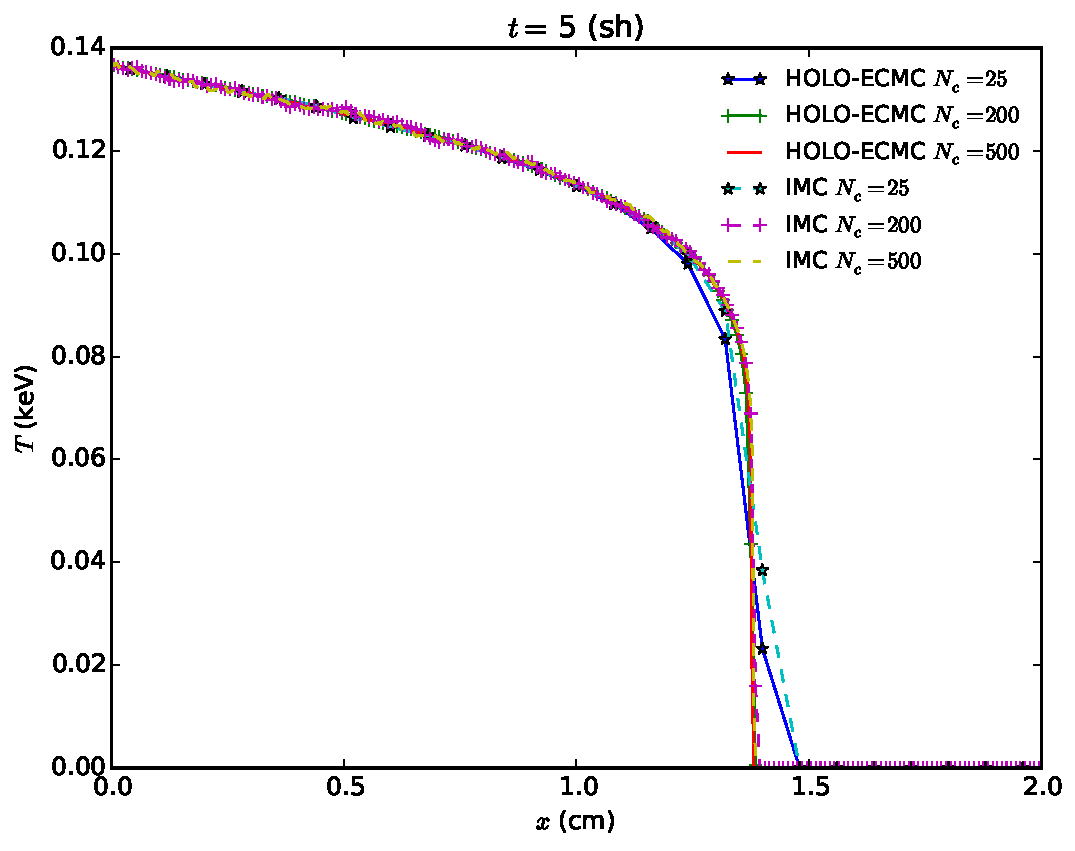
\includegraphics[width=0.99\linewidth]{marshak_mesh_conv.pdf}
    \caption{\label{marshak_mesh_conv} Convergence of IMC and HOLO-ECMC solutions.}
\end{subfigure}
\begin{subfigure}{0.5\textwidth}
  \centering
  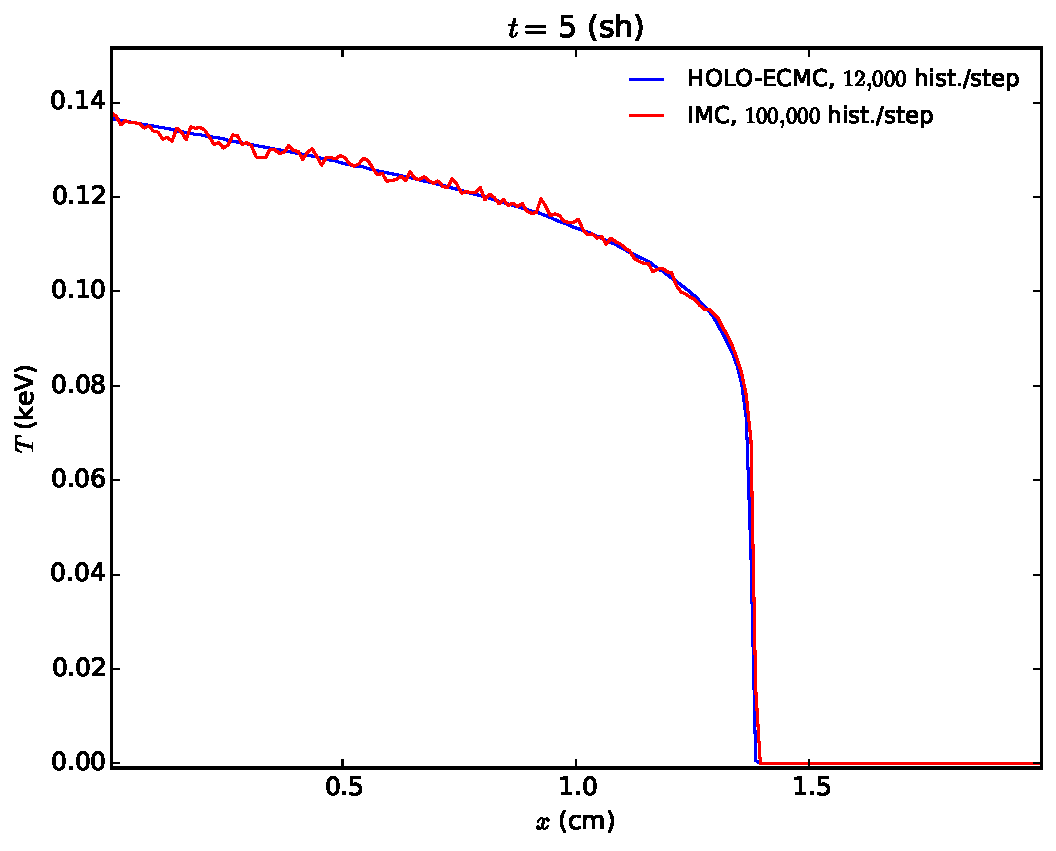
\includegraphics[width=0.99\linewidth]{marshak_200_compare.pdf}
  \caption{\label{marshak_200_compare}  Comparison of solutions for 200 spatial cells. }
\end{subfigure}
\caption{\bf Comparison of solutions for Marshak wave problem at $\mathbf{t=5}$ sh.}
\end{figure}

\Subsection{Two Material Problem}

This problem consists of an optically thin (left) and an optically thick (right) material region,
with constant opacities.  The material properties are given in
Table~\ref{two_mat_props}.  Initially the radiation and material energies are in
equilibrium at a temperature of 0.05 keV.  An isotropic incident intensity of 0.500 keV
is applied at $x=0$ at $t=0$; the isotropic incident intensity on the right boundary is 0.05
keV.  The simulation is ran for 5 sh.

Fig.~\ref{twomat_quick} compares the HOLO and IMC radiation 
temperatures at the end of the simulation. The IMC method used 10$^5$ histories per
time step, where as the HOLO method used $3\times10^4$ histories per time step.  The IMC and HOLO results show agreement
over the finer mesh.
On the coarse mesh ($N_c=25$), the HOLO method predicts the location of the
wave-front more accurately than the IMC method. 

Fig.~\ref{timestep} compares results for different HO solvers.  The HOLO-ECMC results
are for running 3 batches of 10,000 histories, per time step. Also plotted is
the solution for the HOLO method with a standard MC solver as the HO solver
(HOLO-SMC) with
standard source sampling. The SMC
solver uses 10$^5$ histories per time step.  The S$_2$ solution uses the LO
solver with diffusion-equivalent consistency terms and no MC correction.  The HOLO-SMC solution demonstrates significant
statistical noise.  This noise is introduced into the LO solver by bad statistics in
computing the consistency terms. The S$_2$ solution results in an artificially fast
wave front, demonstrating the correction the HO solvers provide.
\begin{table}[htb]
    \begin{center}
        \begin{tabular}{|c|cc|}  \cline{2-3}
            \multicolumn{1}{c|}{}   & $x \in [0,0.5)$ cm & $x \in [0.5,1.0]$ cm   \\ \hline
            $\sigma_a$ (cm$^-1$)  & 0.2 & 2000 \\
            $\rho$ (g cm$^-3$) & 0.03 & 10.0 \\
            $c_v$ (jks/keV-g) & $0.1$ & $0.1$ \\ \hline
        \end{tabular}
        \caption{Two material problem properties \label{two_mat_props}}
    \end{center}
\end{table}

\begin{figure}
\begin{subfigure}{0.5\textwidth}
    \centering
    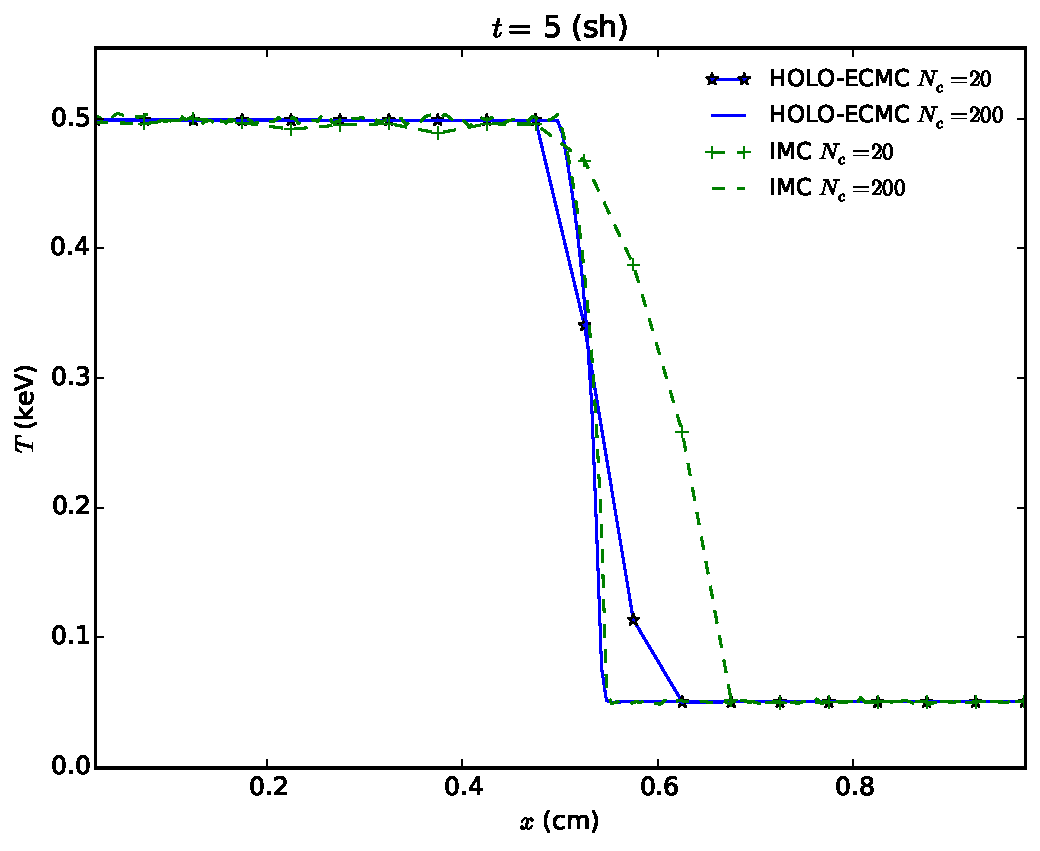
\includegraphics[width=0.99\textwidth]{two_mat_conv.pdf}
    \caption{Comparison of IMC and HOLO-ECMC.\label{twomat_full}}
\end{subfigure}    \begin{subfigure}{0.5\textwidth}
\centering
    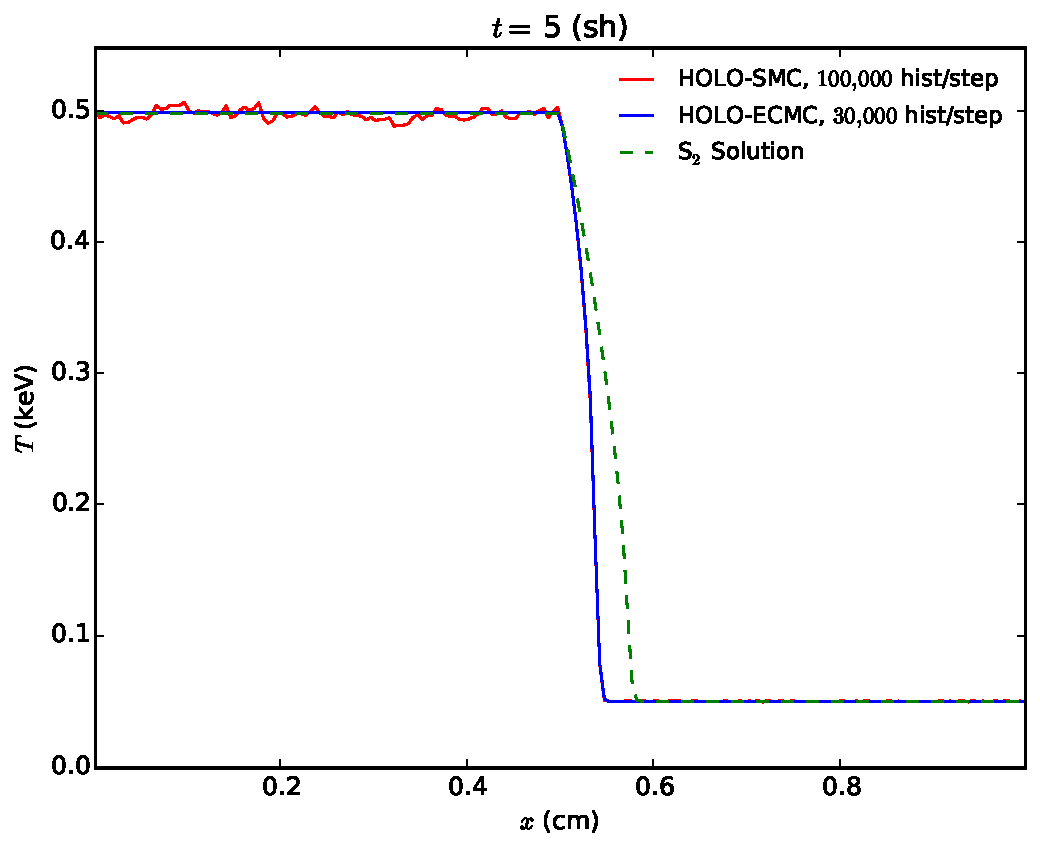
\includegraphics[width=0.99\textwidth]{two_mat_ho_compare.pdf}
    \caption{Comparison of SMC and ECMC HO solvers. \label{twomat_quick}}
\end{subfigure}
    \caption{\bf Comparison of radiation temperatures for two material problem. \label{twomat}}
\end{figure}


\Section{Conclusions}

We have been able to reproduce the IMC solutions for Marshak Wave test problems with
a new HOLO method.  Unlike IMC, our method requires no effective scattering
events to be included in the MC simulation, limiting the total run time of the
simulations; this is also favorable for future parallelization since particles can be
allowed to stream to boundaries without interaction. The LD spatial representation mitigates issues with energy propagating
through the problem artificially fast, similar in effect to source tilting in the IMC
algorithm.   The LO solver resolves the non-linearities in the equations resulting in a fully
implicit time discretization.  The ECMC approach, with initial guesses based on the
previous radiation intensity, results in efficient reduction of statistical error and
allows for particles to be distributed to largely varying regions of the problem.
The LO solver
can accurately and efficiently resolve the solution in diffusive regions, while the HO
transport solver provides the accuracy of a full transport treatment where necessary. 

The primary difficulty to overcome is in the HO
solver at the wave front.  A strictly positive spatial discretization in the HO
system needs to be implemented, e.g., the consistent set to zero method, for high
accuracy solutions. Comparisons to semi-analytic or manufactured solutions will be
performed to demonstrated the benefit of the ECMC iterations for getting
high-accuracy solutions.    Future work will include apllication to multi-frequency 
equations, before extending to multiple spatial dimensions.


\section*{ACKNOWLEDGEMENTS}

This research was performed, in part, using funding received from the DOE Office of Nuclear
Energy's Nuclear Energy University Programs.

\setlength{\baselineskip}{12pt}
%\Section*{REFERENCES}
\bibliographystyle{ans}
\bibliography{references}




\end{document}


